\documentclass[11pt,xcolor=x11names,compress, notes=show]{beamer}% pour l'impression, tout n'apparait qu'une fois \documentclass[handout,12pt]{beamer}
\usepackage[utf8x]{inputenc}
\usepackage{ucs}
\usepackage[UKenglish]{babel}
\usepackage{todonotes}
\usepackage{tikz}
\usepackage{color}
\usepackage{subfigure}
\usetikzlibrary{calc}

\usepackage{bm}
\usepackage{pifont} %pour les symbole sympa \ding{nb}
\usepackage[export]{adjustbox}

\setbeamertemplate{navigation symbols}{} 


%\usepackage{palatino}

%pour le theme
%\usetheme{CambridgeUS}

%\usetheme{Goettingen}
\useinnertheme{default}
\useoutertheme[subsection=false]{miniframes}
\setbeamertemplate{blocks}[rounded][shadow=true]
\setbeamercolor{block title}{fg=DeepSkyBlue4,bg=DeepSkyBlue4!10}
\setbeamercolor{block title alerted}{bg=DeepSkyBlue4!0} 
\setbeamercolor{block title example}{bg=DeepSkyBlue4!20}
\setbeamercolor*{lower separation line head}{bg=DeepSkyBlue4} 

\setbeamerfont{title like}{shape=\scshape}
\setbeamercolor{frametitle}{fg=DeepSkyBlue4}
\setbeamercolor{title}{fg=DeepSkyBlue4}
\setbeamercolor{itemize item}{fg=black}
\setbeamercolor{itemize subitem}{fg=black}
\setbeamercolor{toc}{fg=DeepSkyBlue4}

%couleur table des matières
\usepackage{hyperref}
\hypersetup{colorlinks=true, linkcolor=DeepSkyBlue4}

%Mettre la section courante en titre de diapo (pour champ de titre non-vide)
%\addtobeamertemplate{frametitle}{\frametitle{\insertsubsectionhead}}{}

\addtobeamertemplate{footline}{\hspace{11cm} \insertframenumber/\inserttotalframenumber}

\author{Alice \textsc{Dinsenmeyer} \\~\\ supervised by \\ Romain \textsc{Brossier} \& Ludovic \textsc{Moreau}}

\title{FWI for Ultrasonic Imaging}
\subtitle{Flaw detection in steel weld}
\date{\small \today}

\setbeamertemplate{caption}{\raggedright\insertcaption\par}

\begin{document}

\section{About me}


\begin{frame}
	\begin{center}
		\textbf{Alice \textsc{Dinsenmeyer}}\\
		\footnotesize{PhD student\\[0.5cm]
		\textit{alice.dinsenmeyer@insa-lyon.fr\\
		1\textsuperscript{st} floor, Bât. J. Jacquard}}
			
	\end{center}
	\begin{itemize}
		\item 2011 -- 2014 : BSc in acoustics, Université du Maine, Le Mans %Bachelor of science in acoustics
		\item 2014 --2016 : MSc in acoustics, Université du Maine, Le Mans %Master of science in acoustics
		\begin{columns}
			\hspace{2cm}\column{0.5\textwidth}
			\begin{itemize}
				\item[-] Waves in fluids \& solids
				\item[-] Ultrasonic imaging
				\item[-] Psycho-acoustics
			\end{itemize}
			\column{0.5\textwidth}
			\begin{itemize}
				\item[-] Signal Processing
				\item[-] Computer Science
			\end{itemize}
		\end{columns}
	\end{itemize}
\end{frame}

\section{Thesis}


\begin{frame}
	\centering
	\textbf{ Inverse Method With Bayesian Approach \\for Source Localization in Aeroacoustics}\\
	\footnotesize{started in July, 2017}\\[0.5cm]
	Supervisors : Jérôme Antoni (LVA), Chritophe Bailly (LMFA), Quentin Leclère (LVA)\\[0.5cm]
	Funding : CeLyA + INSAVALOR
\end{frame}

\begin{frame}
	
	
	
\end{frame}

\begin{frame}
	Master internship at Institut des Sciences de la Terre (ISTerre), Grenoble\\
	Full Waveform Inversion for Ultrasonic Imaging,\\
	Flaw detection in steel weld
	
	Détailler context (labo, seiscope, ...)
	
\end{frame}


 \section{Master's Internship}

\section*{NDT for Welds}
\begin{frame}{\insertsectionhead}
\vspace{-0.7cm}
	\begin{figure}
		\centering
		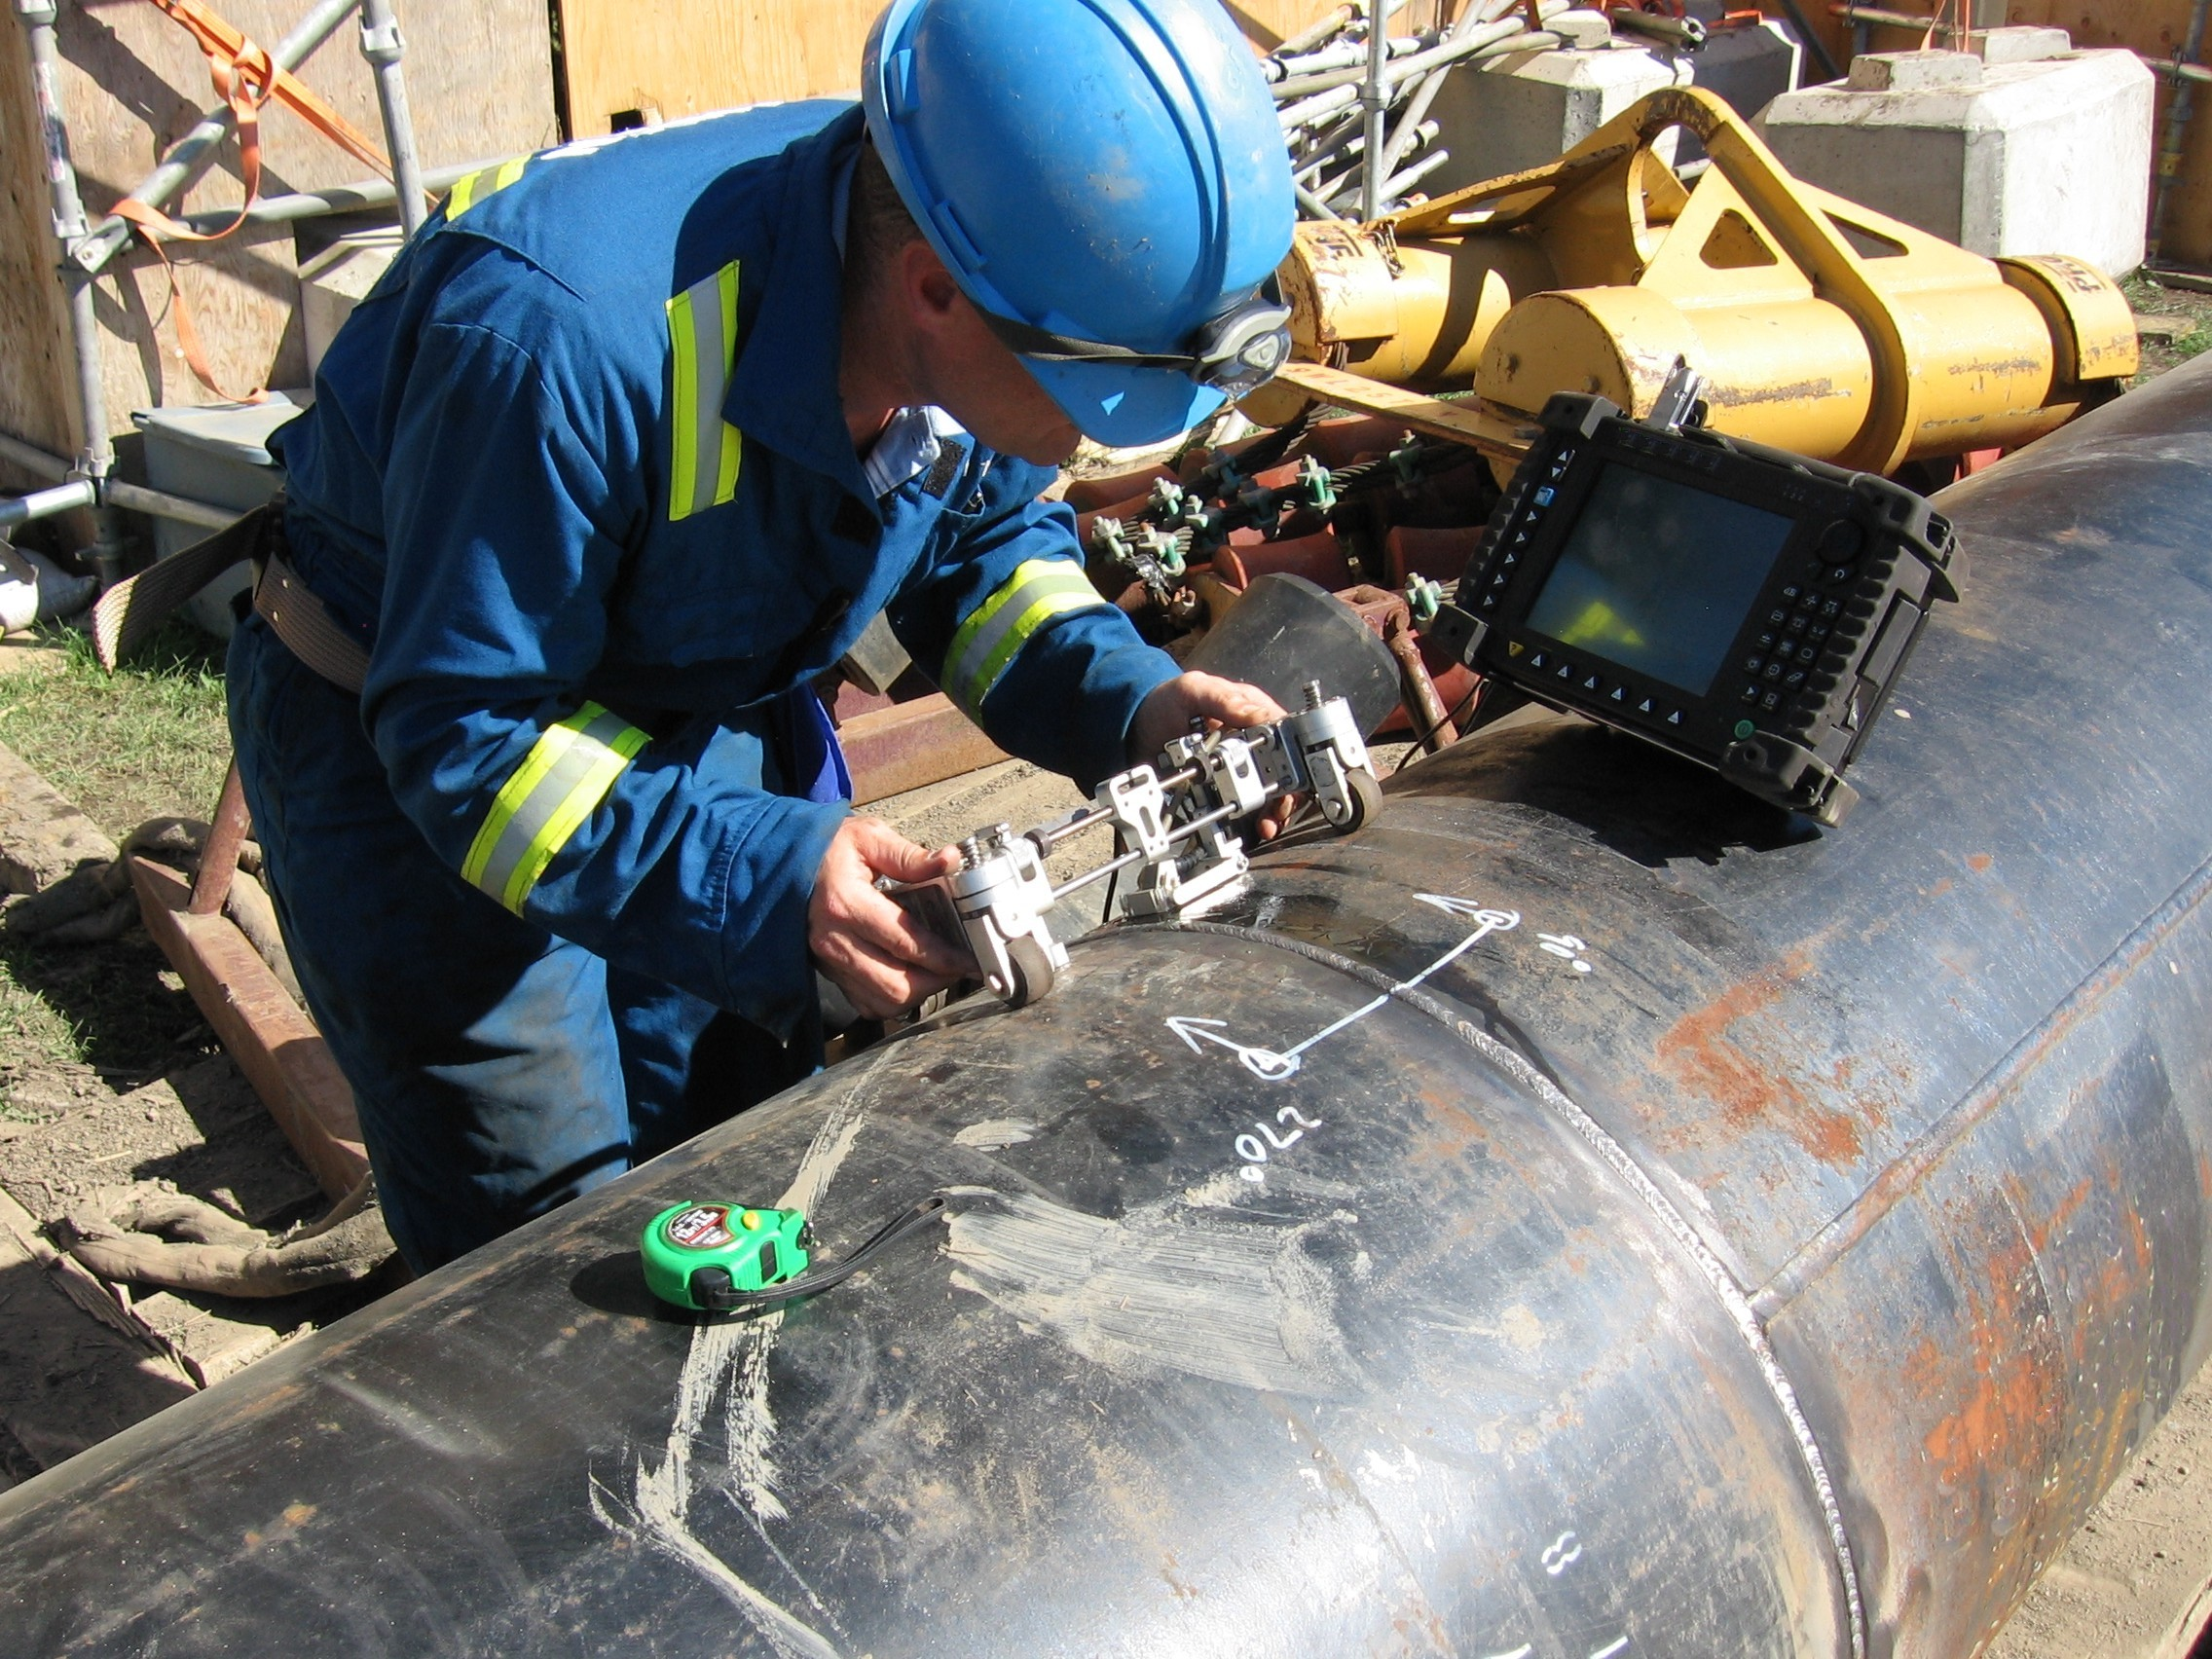
\includegraphics[height=3cm]{img/us_test.jpg}
		\hspace{1cm}
		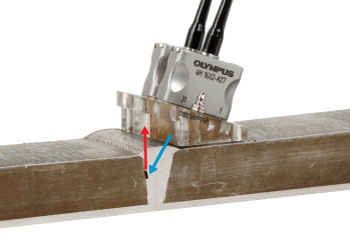
\includegraphics[height=3cm]{img/olympus.jpg}\\
		{\tiny Pipeline test$^{*}$\hspace{4cm} Echo mode testing$^{**}$}
	\end{figure}

	%\begin{columns}
			%\column{.5\textwidth}
			Non destructive testing for weld in :\\
			\begin{itemize}
				\item nuclear reactors (cooling system)
				\item oil and gaz pipelines
			\end{itemize}
			%\column{.05\textwidth}
			%\ding{222}
			%\column{.45\textwidth}
			%\centering
			\vspace{0.6cm}
 			\indent \ding{222} porosity, cracks, lack of fusion, corrosion, inclusions,\ldots
	%\end{columns}


	
\vfill
{\tiny Pictures from $^{*}$Davidmack \& $^{**}$Olympus}\vspace{-0.5cm}
\end{frame}



\begin{frame}{\insertsectionhead}
\vspace{-1cm}
\hspace{1cm}
	\begin{columns}[c]
			\column{.5\textwidth}<1->
			\centering
			\begin{figure}
				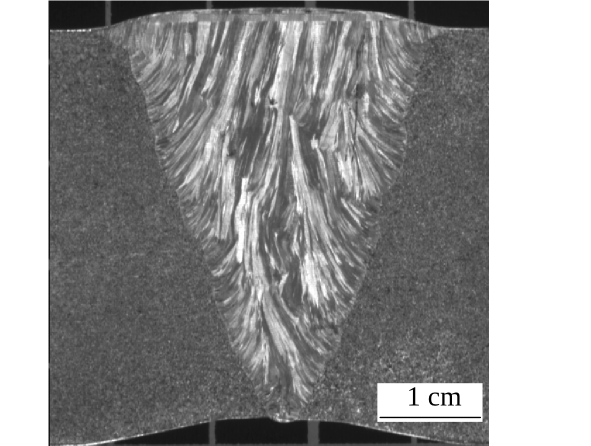
\includegraphics[height=2.7cm]{./img/soudure1.png}\\
				{\centering \tiny Macrography of a weld$^{*}$}
			\end{figure}
			\column{.001\textwidth}<2->
			\hspace{-3cm}
			\vspace{2cm}
			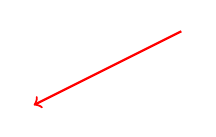
\begin{tikzpicture}
					\draw[<-, thick,shorten <=2pt,shorten >=2pt,red] (-1.5,3)--(0.5,4);
			\end{tikzpicture}
			\column{.9\textwidth}<2->
			%\vfill
			\hspace{-1cm}
			\textcolor{red}{Strong unknown anisotropy}\\
			$\hookrightarrow$ distorsion and splitting of the beam\\[0.2cm]
			\hspace{-0.5cm}
			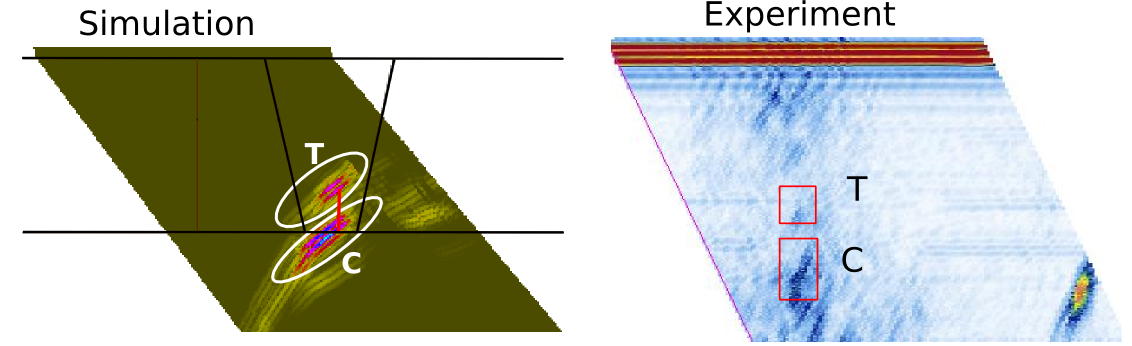
\includegraphics[scale=0.5]{img/gardahaut.png}\\
			{\centering \tiny Comparison of ray based model and experiment result$^{**}$}
				
	\end{columns}
	\vspace{0.3cm}
	\begin{columns}[c]
			\column{.5\textwidth}<1->
			%\begin{block}{}
				\begin{itemize}
					\item[$\bullet$] delay and sum methods
					\item[$\bullet$] decomposition of covariance matrix (DORT)
				\end{itemize}
			%\end{block}
			\column{.05\textwidth}<2->
			\ding{222}
			\column{.5\textwidth}<2->
			%\begin{block}{}
				\begin{itemize}
					\item[\ding{55}] need to know $c$ a priori\\
					\item[\ding{55}] strong artefacts
				\end{itemize}
			%\end{block}
			
	\end{columns}
	\begin{columns}[c]
		\column{.5\textwidth}<3->
			\begin{itemize}
				\item[$\bullet$] solving NL optimization problem
			\end{itemize}
		\column{.05\textwidth}<3->
			\ding{222}
		\column{.5\textwidth}<3->
			\begin{itemize}
			\item contour reconstruction :\\\hspace{-0.5cm}\small{\emph{Dominguez et al.}, \emph{Rodriguez et al.}}\\[0.1cm]
			\item[\ding{51}] \normalsize{$C_{ij}$ reconstruction : FWI}
		\end{itemize}		
	\end{columns}
\vfill
{\tiny Pictures from $^{*}$Chassignole 2000, PhD thesis \& $^{**}$Gardahaut \emph{et al.} 2014}\vspace{-0.5cm}
\end{frame} 

\section{What is specific to weld imaging ?}
\begin{frame}{\insertsectionhead}
	\begin{itemize}
		\item <1-> 2 free surfaces : more information $\leftrightarrow$ non-linear inversion
		\item <2-> surface acquisition only 
		\item <3-> anisotropy $\rightarrow$ multi-parameter inversion \\\hspace{2.3cm}($C_{ij}\times$6 : weld + defects)
		%\item <4-> defects $\rightarrow$ multi-scale inversion ($C_{ij}^{d}\times$6)
	\end{itemize}
	\vfill
	\begin{figure}[!h]
		\centering
		\includegraphics<1-1>[scale=1]{img/soud1.pdf}
		\includegraphics<2-2>[scale=1]{img/soud2.pdf}
		%\includegraphics<3-3>[scale=1]{img/soud3.pdf}
		\includegraphics<3-3>[scale=1]{img/soud4_bis.pdf}
	\end{figure}

\end{frame}

%\section{To do}
%\begin{frame}{\insertsectionhead}
%	\begin{itemize}
%		\item <1-> 2D acoustic approximation (mono/multiparameter)
%		\begin{itemize}
%			\item isotropic weld ($v_{p}$, $\rho$)
%			\item transverse isotropic weld ($v_{p}$, $\rho$, $\epsilon$, $\delta$, $\theta$)
%		\end{itemize}
%		\item <2-> 3D elastic inversion (mono/multiparameter : $C_{ij}\times$6)
%		\begin{itemize}
%			\item isotropic weld
%			\item anisotropic weld
%			\item real data
%		\end{itemize}		
%	\end{itemize}
%\end{frame}

\section{To do}
\begin{frame}{\insertsectionhead}
	\begin{itemize}
		\item 2D acoustic approximation (mono/multiparameter)
		\begin{itemize}
			\item isotropic weld (\fcolorbox{DeepSkyBlue4}{DeepSkyBlue4!10}{$v_{p}$}, \fcolorbox{DeepSkyBlue4}{DeepSkyBlue4!10}{$\rho$})
			\item transverse isotropic weld ($v_{p}$, $\rho$, \fcolorbox{DeepSkyBlue4}{DeepSkyBlue4!10}{$\epsilon$}, $\delta$, $\theta$)
		\end{itemize}
		\item 3D elastic inversion (mono/multiparameter : $C_{ij}\times$6)
		\begin{itemize}
			\item isotropic weld : \fcolorbox{DeepSkyBlue4}{DeepSkyBlue4!10}{$v_{p}$}
			\item anisotropic weld
			\item real data
		\end{itemize}		
	\end{itemize}
\end{frame}

\begin{frame}
	\begin{columns}
		\column{.7\textwidth}
		\begin{figure}[!h]
			\flushleft
			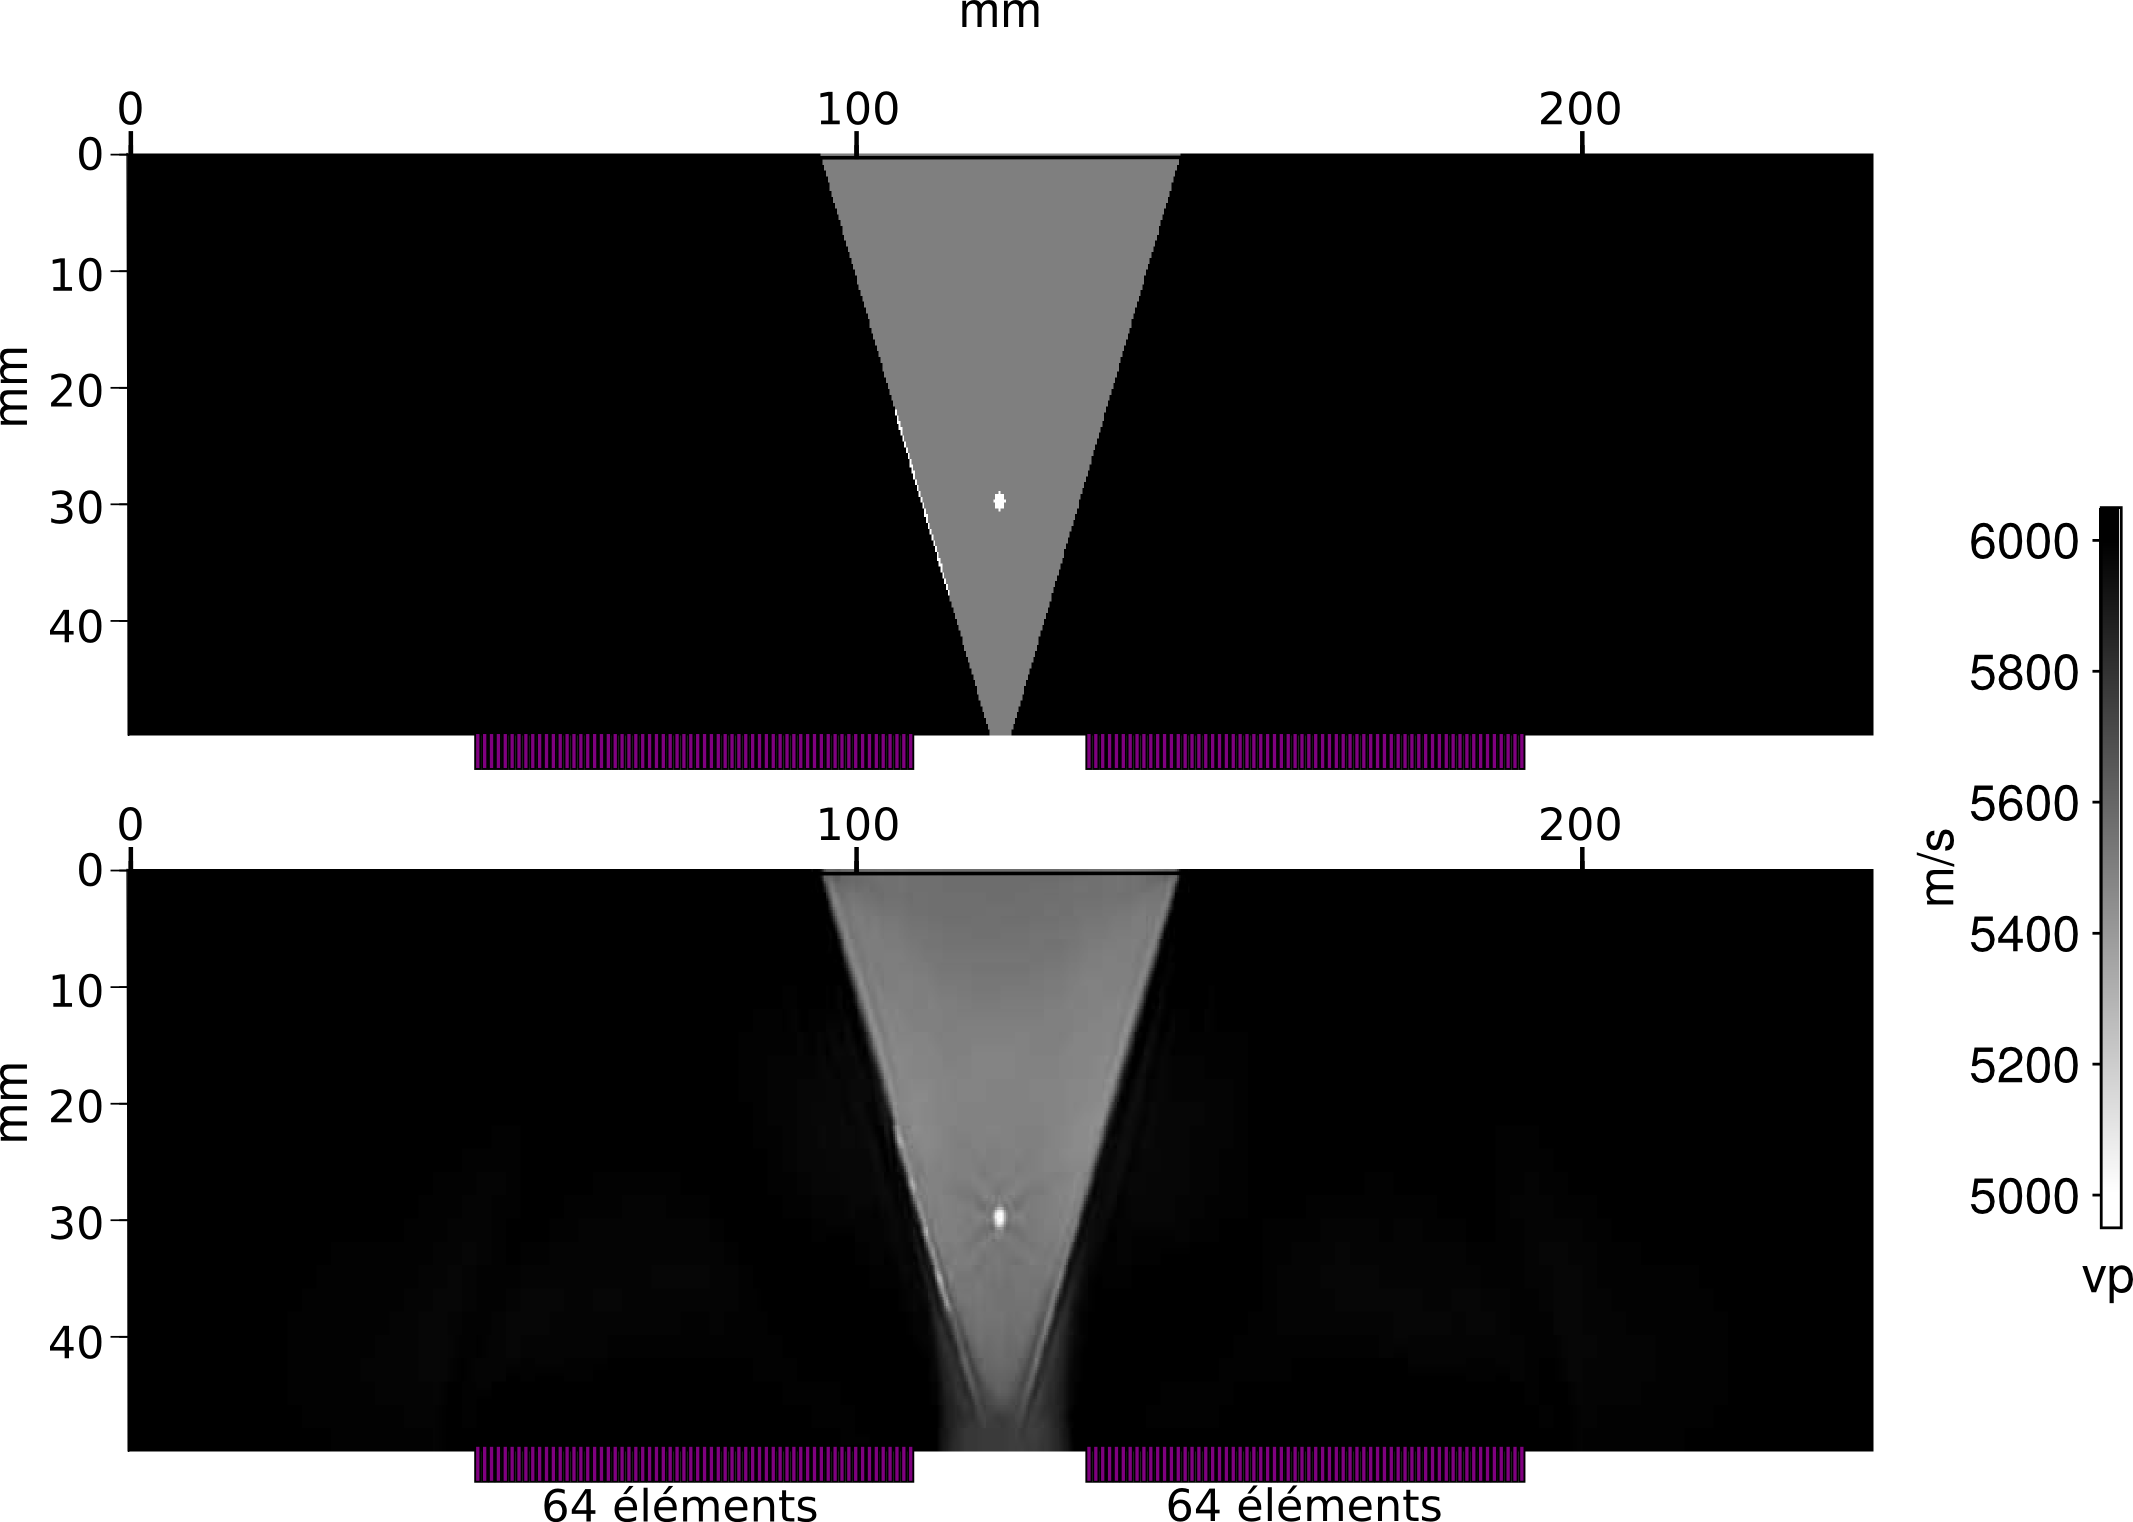
\includegraphics[width=\textwidth]{img/vp.png}\\[0.5cm]
		\end{figure}
		\vline
		\column{.36\textwidth}
		\begin{figure}[!h]
			\flushright
			\vspace{-1cm}
			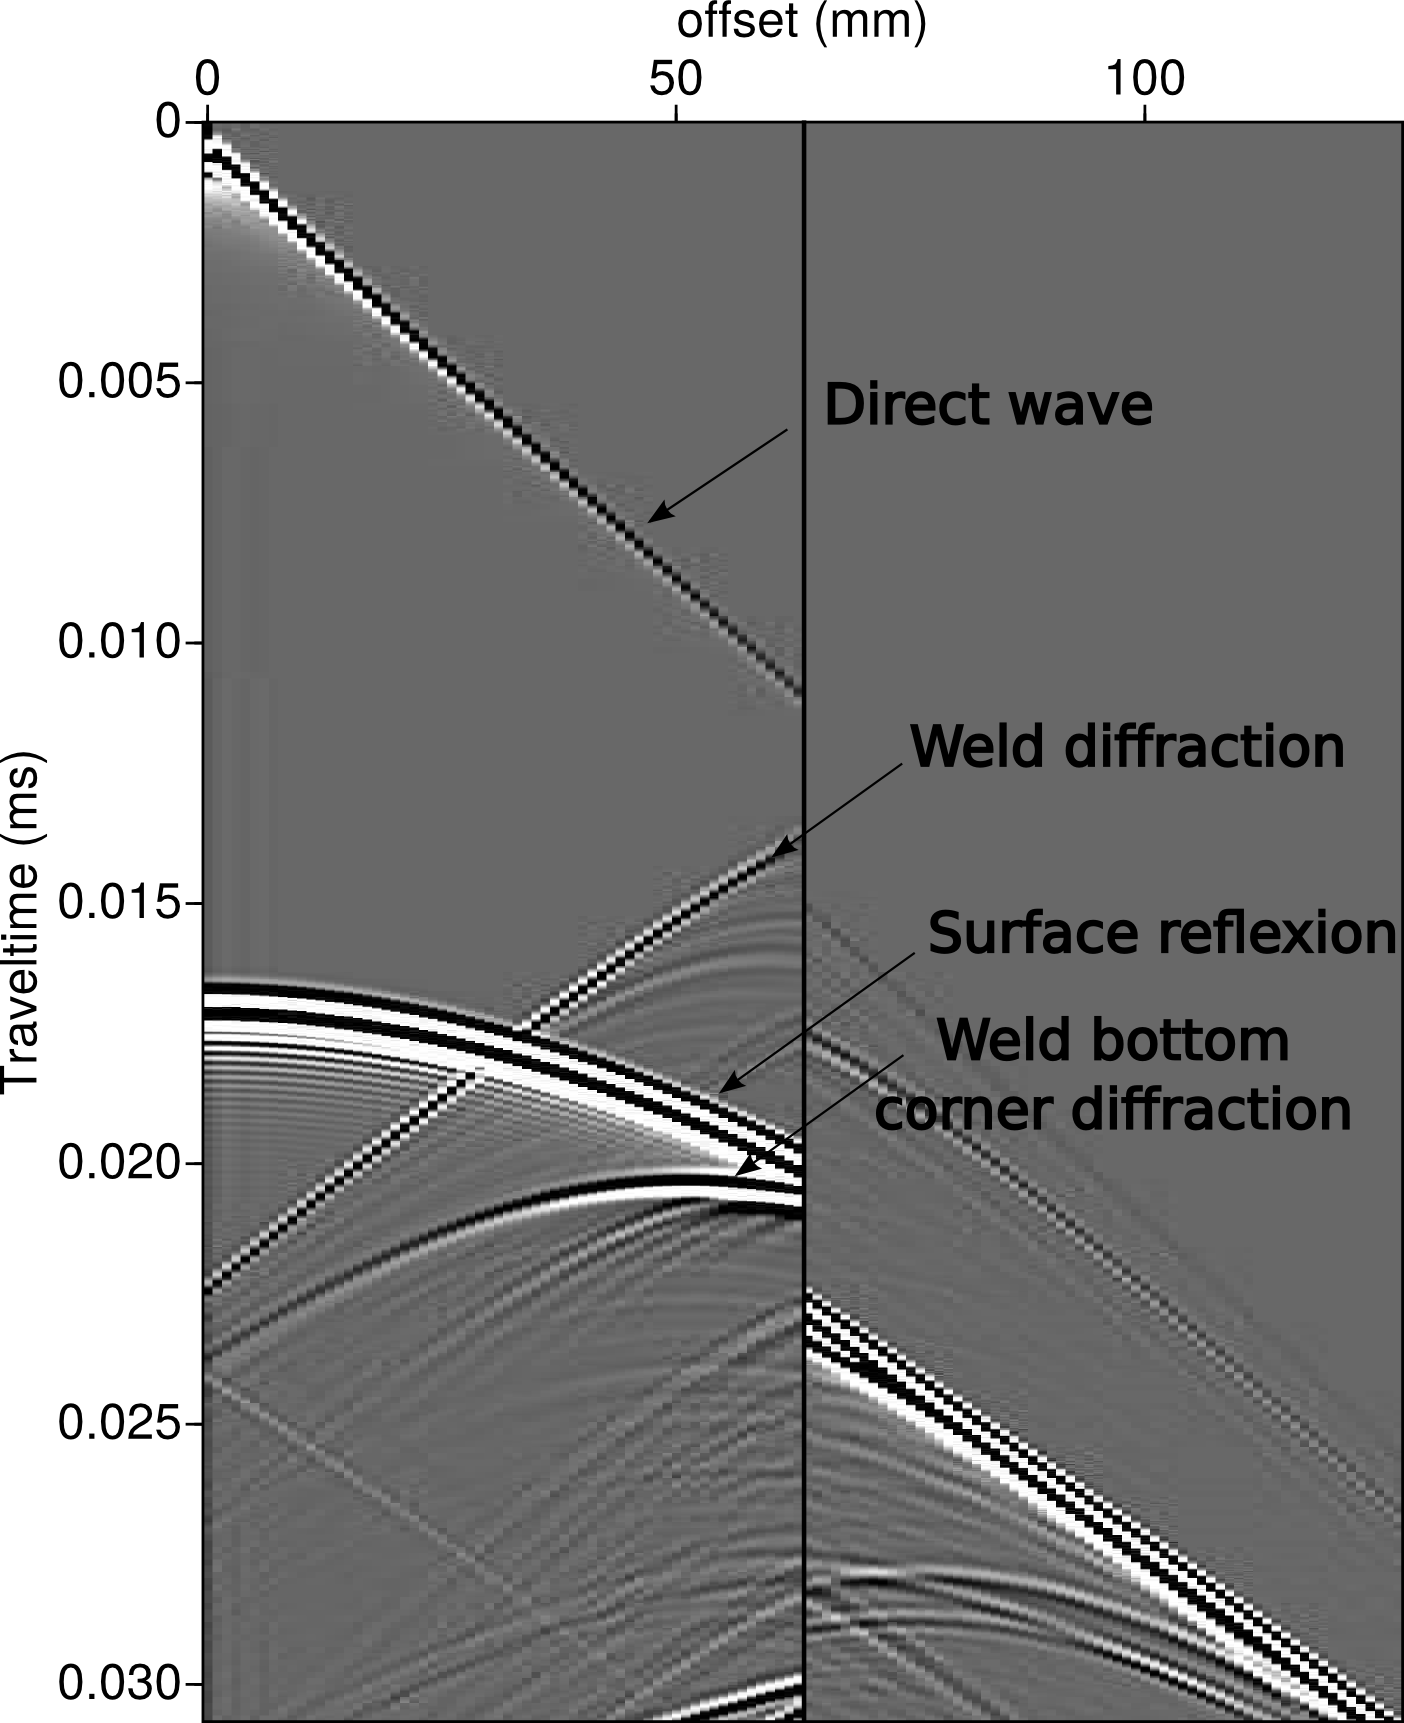
\includegraphics[width=\textwidth]{img/ondes.png}
		\end{figure}
	\end{columns}
	\begin{center}
			2D isotropic case :  monoparameter inversion of $v_{p}$\\ 100kHz $\rightarrow$5MHz
	\end{center}

\end{frame}

\section{To do}
\begin{frame}{\insertsectionhead}
	\begin{itemize}
		\item 2D acoustic approximation (mono/multiparameter)
		\begin{itemize}
			\item isotropic weld (\fcolorbox{DeepSkyBlue4}{DeepSkyBlue4!10}{$v_{p}$}, \fcolorbox{DeepSkyBlue4}{DeepSkyBlue4!10}{$\rho$})
			\item transverse isotropic weld ($v_{p}$, $\rho$, \fcolorbox{DeepSkyBlue4}{DeepSkyBlue4!10}{$\epsilon$}, $\delta$, $\theta$)
		\end{itemize}
		\item 3D elastic inversion (mono/multiparameter : $C_{ij}\times$6)
		\begin{itemize}
			\item isotropic weld : \fcolorbox{DeepSkyBlue4}{DeepSkyBlue4!10}{$v_{p}$}
			\item anisotropic weld
			\item real data
		\end{itemize}		
	\end{itemize}
\end{frame}

\end{document}